\chapter{適用例}\label{cha:Indication}
本章では、適用例を用いて、今回試作した\toolName が正しく動作することを確認する。
\toolName が変更前のWebページのURLと、変更後のWebページのURLを入力として、
以下に示す8つのPNG形式の画像を生成する。
\begin{itemize}
    \item 変更前画像:\\
          Webページの変更前画像
    \item 変更後画像:\\
          Webページの変更後画像
    \item 差分箇所変更前画像:\\
          変更により削除された範囲を、赤枠で囲むことで強調表示した、Webページの変更前画像
    \item 差分箇所変更後画像:\\
          変更により追加された範囲を、緑枠で囲むことで強調表示した、Webページの変更後画像
    \item 変更箇所変更前画像:\\
          変更により削除された画面要素の範囲を、赤枠で囲むことで強調表示した、Webページの変更前画像
    \item 変更箇所変更後画像:\\
          変更により追加された画面要素の範囲を、緑枠で囲むことで強調表示した、Webページの変更後画像
    \item 不具合箇所変更前画像:\\
          レイアウトの不具合箇所のうち、HTMLコードに基づいて削除されていない範囲を、赤枠で囲むことで強調表示した、Webページの変更前画像
    \item 不具合箇所変更後画像:\\
          レイアウトの不具合箇所のうち、HTMLコードに基づいて追加されていない範囲を、緑枠で囲むことで強調表示した、Webページの変更後画像
\end{itemize}
今回の検証を行うために、以下のWebページを用意する。
\begin{itemize}
    \setlength{\itemsep}{0pt}
          \setlength{\parsep}{0pt}
    \item テスト対象とするWebページA\label{item: ex1_bf}
    \item AのWebページに対して、レイアウトの不具合が発生するよう変更したWebページB\label{item: ex1_af}
\end{itemize}
なお、WebページAに対して、以下の変更を行った。
\begin{enumerate}[label=変更\arabic*., leftmargin=1.8cm]
    \item 「有留大学」を「有留大学 受講科目登録」に変更\label{item: Act1}
    \item ログインフォームのロゴを追加\label{item: Act2}
    \item パスワード欄とログインボタンの間に「フリーWi-Fiでのログインに関する注意書き」のテキストを追加\label{item: Act3}
    \item 「有留大学情報基盤センター」のリンクを削除\label{item: Act4}
\end{enumerate}
テスト対象とするWebページAを図\ref{fig:bf_original}に、
図\ref{fig:bf_original}のWebページAにレイアウトの不具合箇所が発生するよう変更したWebページBを図\ref{fig:af_original}に、
それぞれ示す。
% 以降、上記の2つのWebページを適用例に用いて、レイアウトの不具合箇所を可視化できることを確認する。
\begin{figure}[htbp]
    \centering
    % 画像ファイル名とサイズを指定
    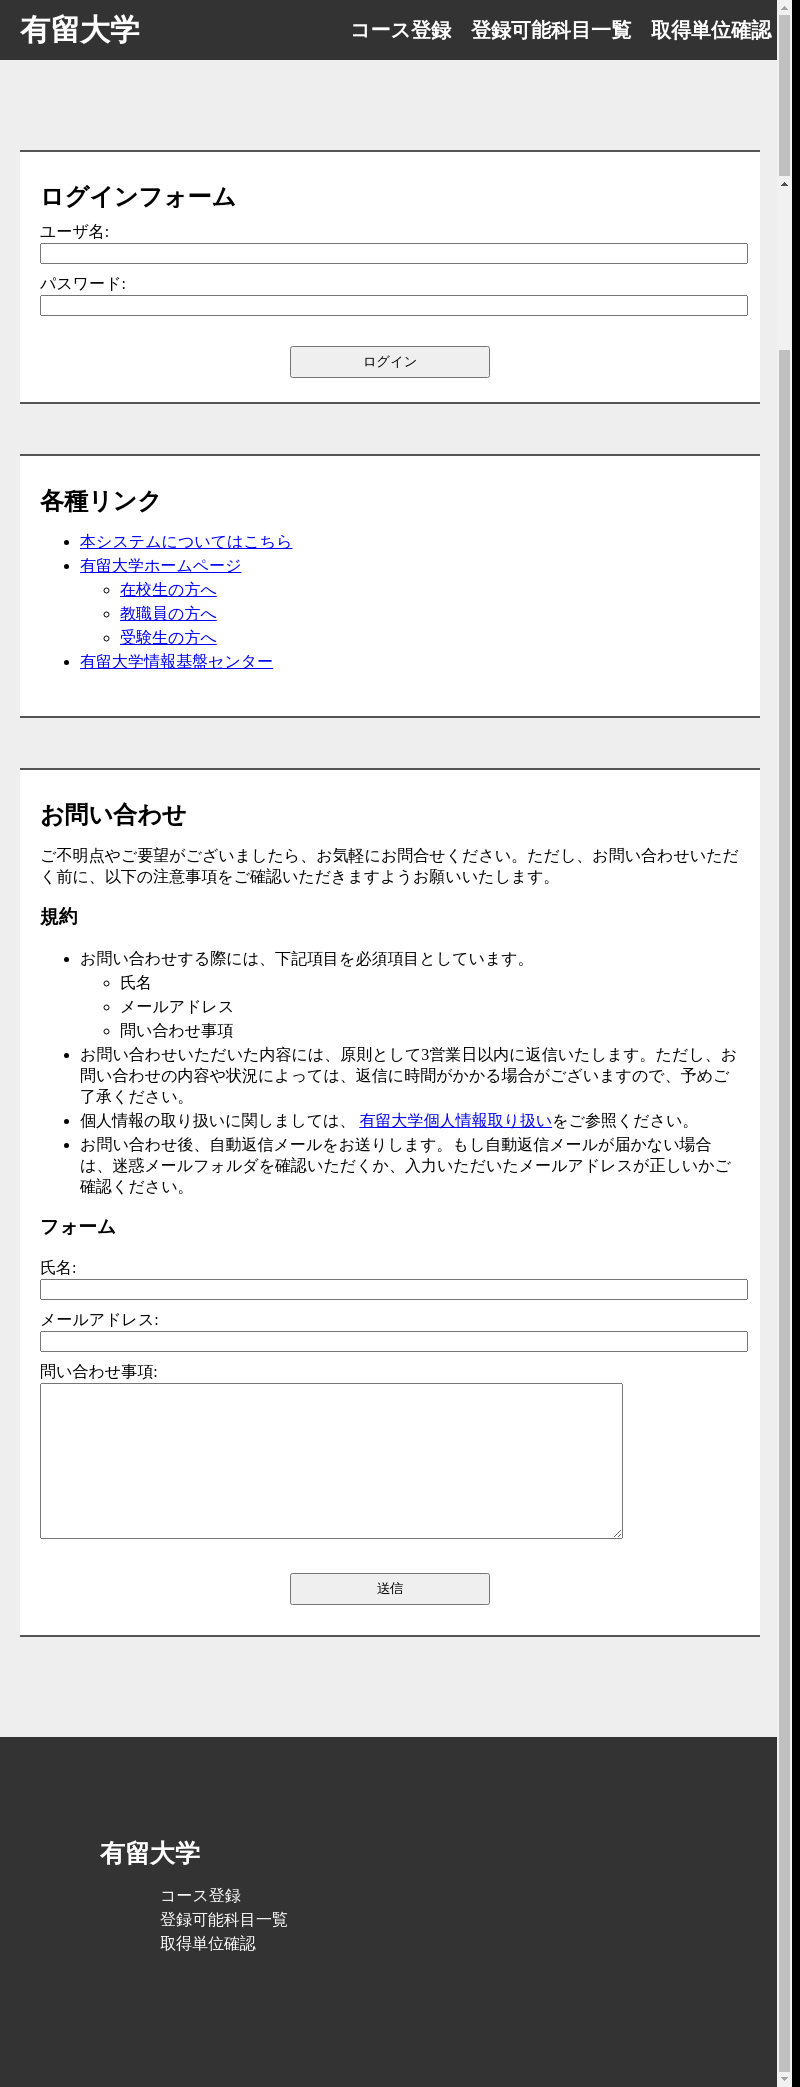
\includegraphics[width=0.5\textwidth]{image/5/original_png/bf_original.png}
    \caption{テスト対象とするWebページA}
    \label{fig:bf_original}
\end{figure}
\begin{figure}[htbp]
    \centering
    % 画像ファイル名とサイズを指定
    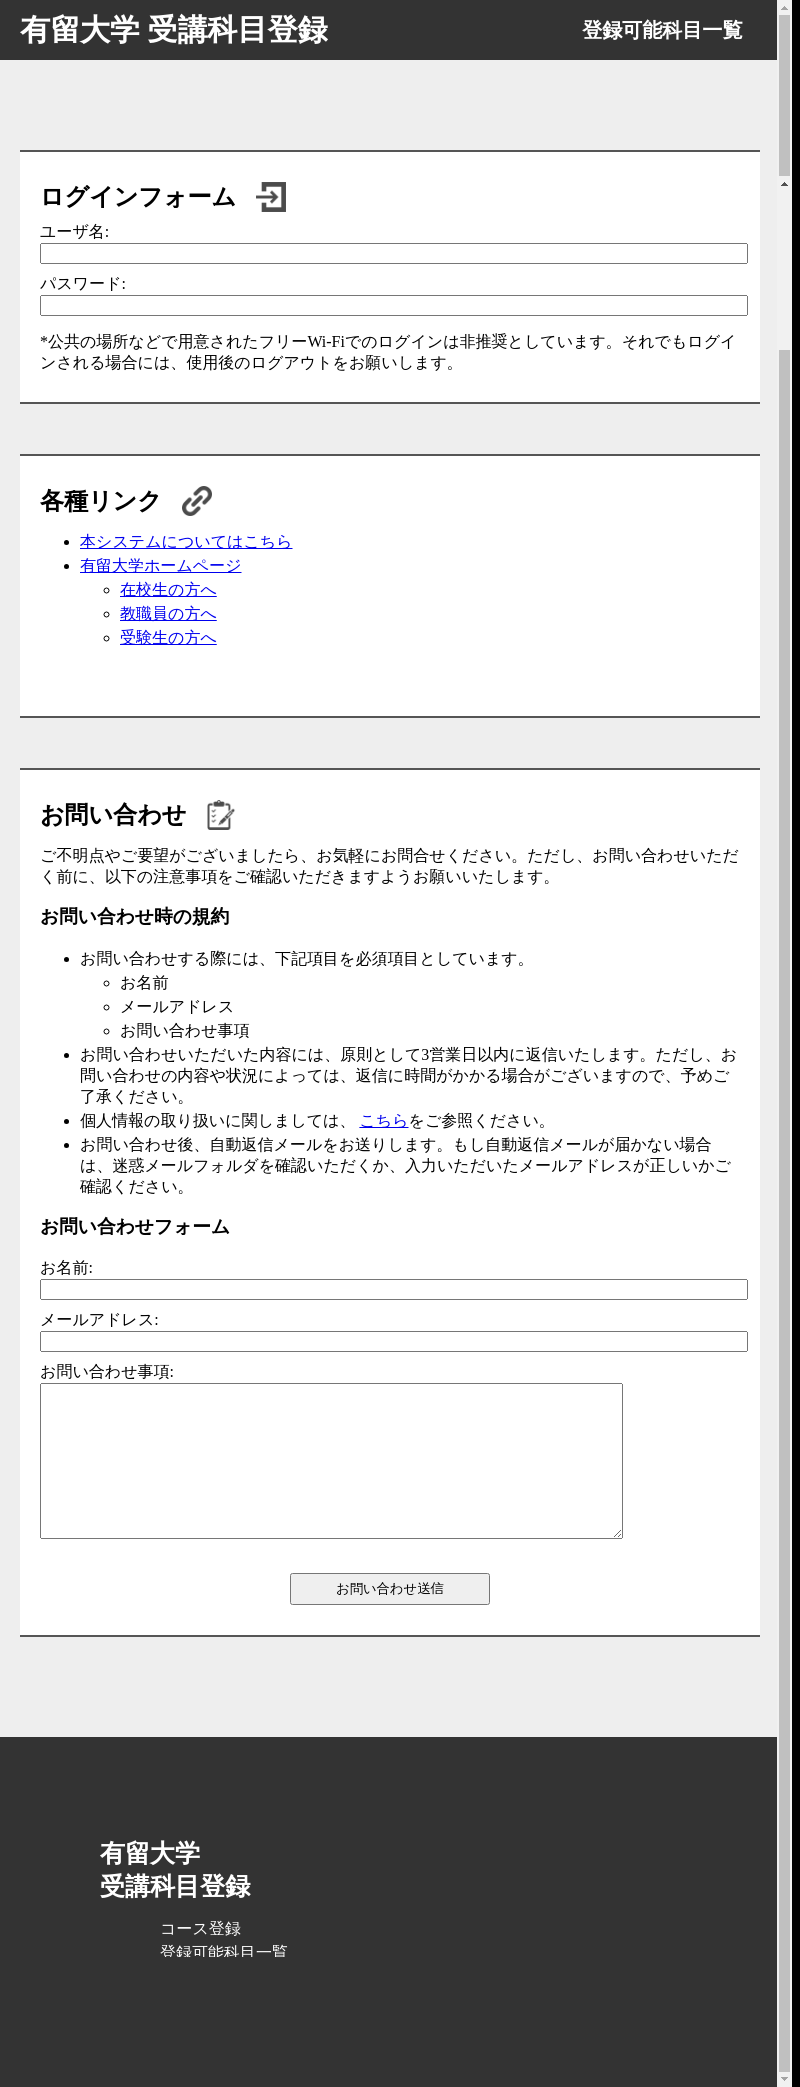
\includegraphics[width=0.5\textwidth]{image/5/original_png/af_original.png}
    \caption{図\ref{fig:bf_original}のWebページAにレイアウトの不具合が発生するよう変更したWebページB}
    \label{fig:af_original}
\end{figure}

以降の節では、適用例を用いて、\toolName が特定する3つの範囲を正常に強調表示できることを確認する。
% 画像比較に基づく差分箇所表示、HTMLコードの変更に基づく変更箇所表示、レイアウトの不具合箇所表示
% のそれぞれの
% 画像比較に基づく差分箇所からHTMLコードに基づかないレイアウトの不具合箇所を
% 可視化できることを確認する。
% \toolName のUIは、以下に示す4つのを持つメニューと、各に対応するコンテンツからなる。
% \begin{itemize}
%     \item[①] メニュー
%           \begin{itemize}
%               \item オリジナル表示
%               \item 画像比較に基づく差分箇所表示
%               \item HTMLコードの変更に基づく変更箇所表示
%               \item レイアウトの不具合箇所表示
%           \end{itemize}
%     \item[②] コンテンツ
% \end{itemize}
% \par
% \toolName を用いて、HTMLコードに基づかないレイアウトの不具合箇所を可視化できるかどうかを確認するために、以下の4つのパターンについて確認する。
% \begin{itemize}
%     \item  画像比較に基づく差分箇所表示通りにHTMLコードに基づく変更箇所に削除されている
%     \item 画像比較に基づく差分箇所表示通りにHTMLコードに基づく変更箇所に削除されていない
%     \item 画像比較に基づく差分箇所表示通りにHTMLコードに基づく変更箇所に追加されている
%     \item 画像比較に基づく差分箇所表示通りにHTMLコードに基づく変更箇所に追加されていない
% \end{itemize}
% \par

\section{画像比較に基づく差分箇所表示の確認}
適用例を用いて、画像比較に基づく差分箇所表示が、正しく行われていることを確認する。
図\ref{fig:bf_original}と図\ref{fig:af_original}の適用例における画像の比較に基づく差分箇所表示を、図\ref{fig: 5_app2}に示す。
画像比較に基づく差分箇所表示における赤枠は削除された範囲を示し、緑枠は追加された範囲を示す。
図\ref{fig: 5_app2}を見ると、
変更前画像上で赤枠で囲まれている「コース登録」は、変更後画像上には存在しない。
よって、変更後に削除された「コース登録」が変更前画像上で正しく赤枠で囲まれていることを確認できる。
また、
変更後画像上で緑枠で囲まれている「登録可能科目一覧」は、変更前画像上に存在するが、同じ位置に存在しない。
よって、変更後に追加された「登録可能科目一覧」が変更後画像上で正しく緑枠で囲まれていることを確認できる。
\par
以上のことから、
画像比較に基づく差分箇所表示が、正しく行われていることを確認できる。
\begin{figure}[tp]
    \begin{center}
        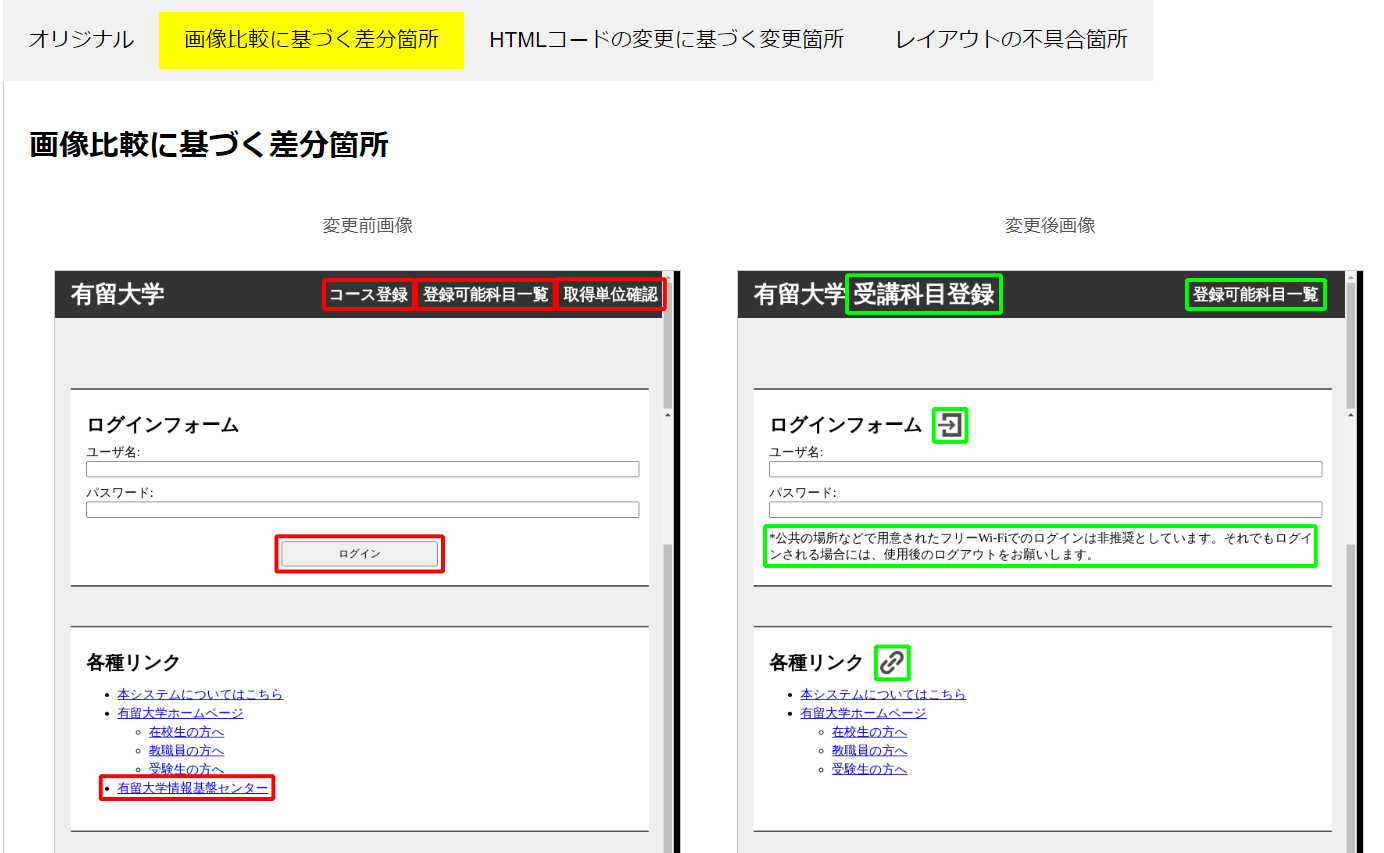
\includegraphics[width=1.0\columnwidth]{image/5/new_img.png}
        \caption{図\ref{fig:bf_original}と図\ref{fig:af_original}における画像比較に基づく差分箇所表示}
        \label{fig: 5_app2}
    \end{center}
\end{figure}



\section{HTMLコードの変更に基づく変更箇所表示の確認}
適用例を用いて、HTMLコードの比較に基づく変更箇所表示が、正しく行われていることを確認する。
図\ref{fig:bf_original}と図\ref{fig:af_original}の適用例における変更箇所表示を、図\ref{fig: 5_app1}に示す。
HTMLコードの比較に基づく変更箇所表示における赤枠は削除された画面要素の範囲を示し、緑枠は追加された画面要素の範囲を示す。
図\ref{fig: 5_app1}を見ると、
変更前画像上で「有留大学」が赤枠で囲まれており、
変更後画像上で「有留大学 受講科目登録」が緑枠で囲まれている。
これは、\ref{item: Act1}と照らし合わせると、
赤枠で囲まれた「有留大学」は削除され、緑枠で囲まれた「有留大学 受講科目登録」は追加されたことを確認できる。
一方で、\ref{item: Act1}~\ref{item: Act4}における変更対象ではない、「コース登録」や「登録可能科目一覧」などに対しては、
赤枠や緑枠で囲まれていないことを確認できる。
\par
以上のことから、
HTMLコードの変更に基づく変更箇所表示が、正しく行われていることを確認できる。
\begin{figure}[tp]
    \begin{center}
        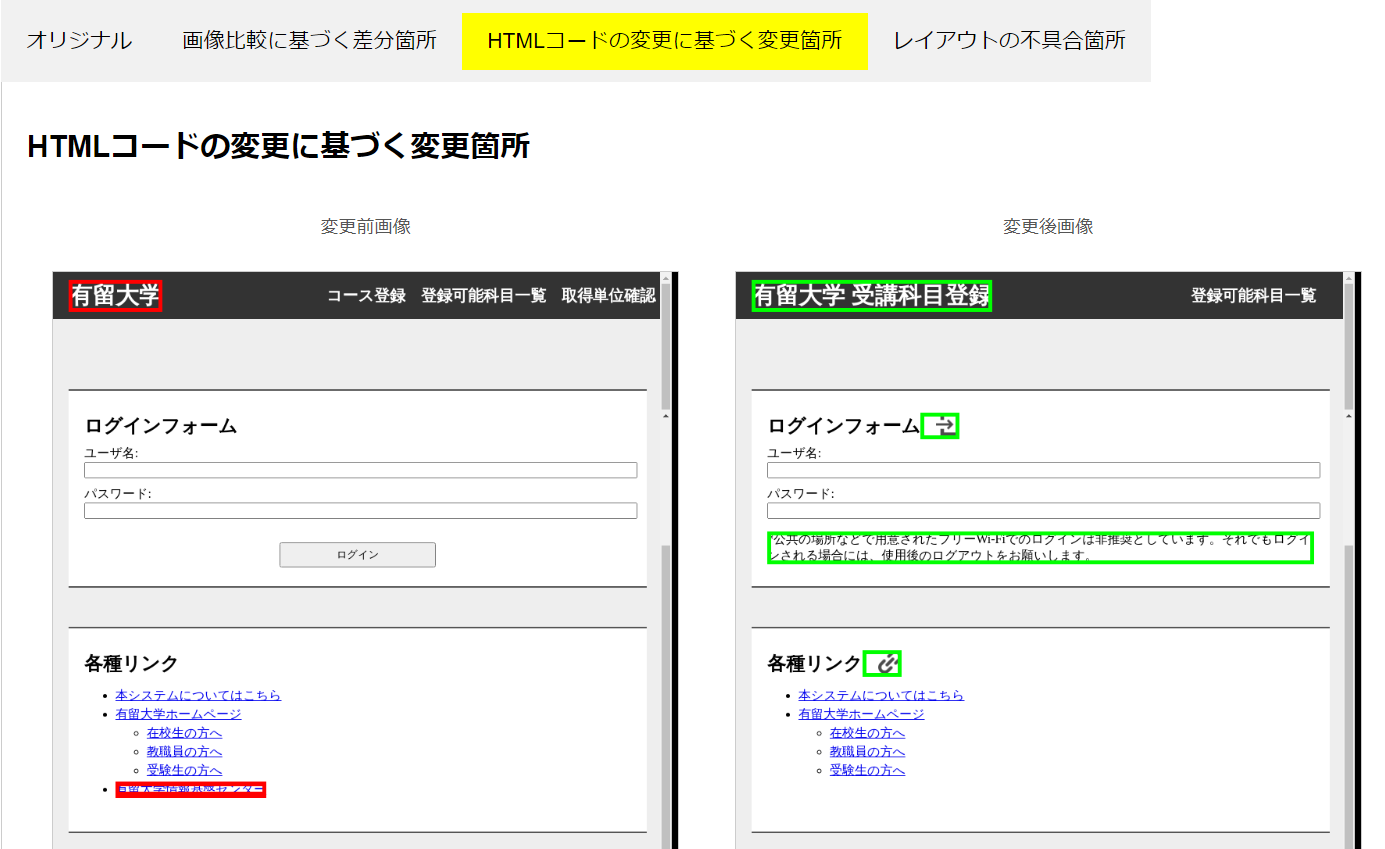
\includegraphics[width=1.0\columnwidth]{image/5/new_html.png}
        \caption{図\ref{fig:bf_original}と図\ref{fig:af_original}の適用例におけるHTMLコードの比較に基づく変更箇所表示}
        \label{fig: 5_app1}
    \end{center}
\end{figure}


\section{レイアウトの不具合箇所表示の確認}
適用例を用いて、レイアウトの不具合箇所表示が、正しく行われていることを確認する。
図\ref{fig:bf_original}と図\ref{fig:af_original}の適用例におけるレイアウトの不具合箇所表示を、図\ref{fig: 5_app3}に示す。
HTMLコードに基づかないレイアウトの不具合箇所を確認するために、以下の4つのパターンについて確認する。
\begin{itemize}
    \item 画像比較に基づく差分箇所表示通りに画面要素が削除されている
    \item 画像比較に基づく差分箇所表示通りに画面要素が削除されていない
    \item 画像比較に基づく差分箇所表示通りに画面要素が追加されている
    \item 画像比較に基づく差分箇所表示通りに画面要素が追加されていない
\end{itemize}
以降、レイアウトの不具合箇所表示が、正しく行われていることを確認する。
\begin{figure}[tp]
    \begin{center}
        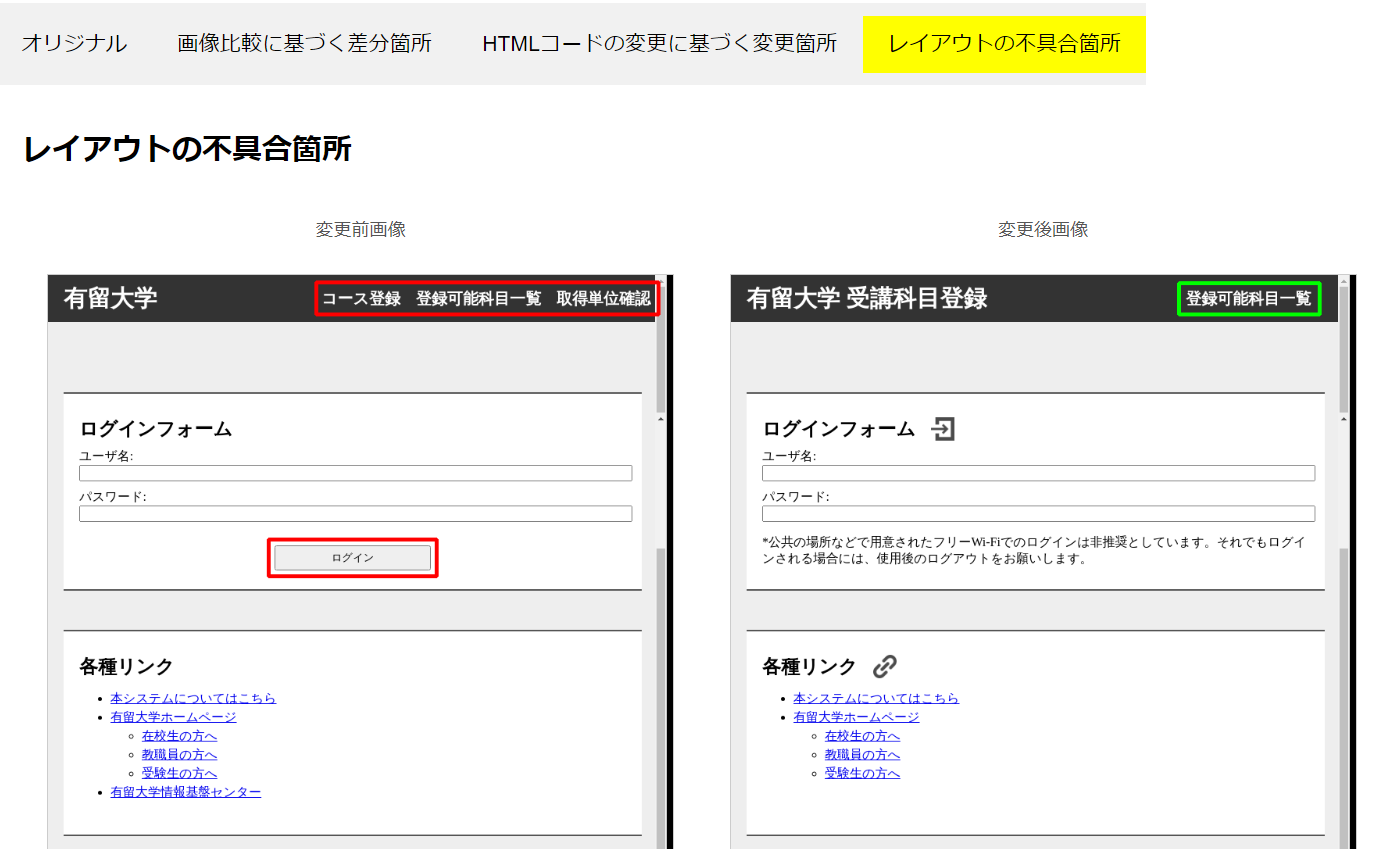
\includegraphics[width=1.0\columnwidth]{image/5/new_effect.png}
        \caption{図\ref{fig:bf_original}と図\ref{fig:af_original}の適用例におけるレイアウトの不具合箇所表示}
        \label{fig: 5_app3}
    \end{center}
\end{figure}




\subsection{パターン1: 画像比較に基づく差分箇所表示通りに画面要素が削除されている}\label{sec:result_area_detection}
適用例を用いて、画像比較に基づく差分箇所表示通りに画面要素が削除されていることを確認する。
図\ref{fig: 5_app2}の画面を確認すると、変更前画像上の一番下のリンクが赤枠で囲まれていることが分かる。
この赤枠に着目すると、赤枠は変更後画像上で削除されていることが分かる。
次に、画像比較に基づく差分箇所表示通りに削除されているかどうかを確かめるために、
図\ref{fig: 5_app1}のHTMLコードの比較に基づく変更箇所表示を確認すると、
赤枠で囲まれているため、HTMLコードに基づいて削除された箇所だと分かる。
最後に、図\ref{fig: 5_app3}のレイアウトの不具合箇所表示で確認すると、
レイアウトの不具合箇所として赤枠で囲まれていないことが分かる。
\par
よって、\toolName を用いることで、画像比較に基づく差分箇所表示通りに削除されていることを確認できる。



\subsection{パターン2: 画像比較に基づく差分箇所表示通りに画面要素が削除されていない}\label{sec:result_area2}
適用例を用いて、画像比較に基づく差分箇所表示通りに画面要素が削除されていないことを確認する。
図\ref{fig: 5_app2}の画面を確認すると、変更前画像上のログインボタンが赤枠で囲まれていることが分かる。
この赤枠に着目すると、変更後画像上で削除されていることが分かる。
次に、画像比較に基づく差分箇所表示通りに削除されているかどうかを確かめるために、
図\ref{fig: 5_app1}のHTMLコードの比較に基づく変更箇所表示を確認すると、
赤枠で囲まれていないため、HTMLコードに基づいて削除されていない箇所だと分かる。
このことから、緑枠で囲まれたテキストによって、ログインボタンが隠れた状態になっていると推測できる。
最後に、図\ref{fig: 5_app3}のレイアウトの不具合箇所表示で確認すると、
レイアウトの不具合箇所として赤枠で囲まれていることが分かる。
\par
よって、\toolName を用いることで、画像比較に基づく差分箇所表示通りに画面要素が削除されていないことを確認できる。


\subsection{パターン3: 画像比較に基づく差分箇所表示通りに画面要素が追加されている}\label{sec:result_area3}
適用例を用いて、画像比較に基づく差分箇所表示通りに画面要素が追加されていることを確認する。
図\ref{fig: 5_app2}の画面を確認すると、変更後画像上の左上テキスト「受講科目登録」が緑枠で囲まれていることが分かる。
この緑枠に着目すると、変更前画像上から追加されていることが分かる。
次に、差分箇所表示通りに追加されているかどうかを確かめるために、
図\ref{fig: 5_app1}のHTMLコードの比較に基づく変更箇所表示を確認すると、
緑枠で囲まれているため、HTMLコードに基づいて追加された箇所だと分かる。
最後に、図\ref{fig: 5_app3}のレイアウトの不具合箇所表示で確認すると、
レイアウトの不具合箇所として緑枠で囲まれていないことが分かる。
\par
よって、\toolName を用いることで、画像比較に基づく差分箇所表示通りに画面要素が追加されていることを確認できる。


\subsection{パターン4: 画像比較に基づく差分箇所表示通りに画面要素が追加されていない}\label{sec:result_area4}
適用例を用いて、画像比較に基づく差分箇所表示通りに画面要素が追加されていないことを確認する。
図\ref{fig: 5_app2}の画面を確認すると、変更後画像上の右上テキスト「登録可能科目一覧」が緑枠で囲まれていることが分かる。
この緑枠に着目すると、緑枠内のテキストと完全一致するテキストが変更前画像上に赤枠で囲まれているため、
変更前画像上から削除され、変更後画像上に新しく追加されていることが分かる。
% つまり、変更後にテキストの配置の変更があったと推測できる。
次に、差分箇所表示通りに追加されているかどうかを確かめるために、
図\ref{fig: 5_app1}のHTMLコードの比較に基づく変更箇所表示を確認すると、
緑枠で囲まれていないため、HTMLコードに基づいて追加されていない箇所だと分かる。
最後に、図\ref{fig: 5_app3}のレイアウトの不具合箇所表示で確認すると、
レイアウトの不具合箇所として緑枠で囲まれていることが分かる。
\par
よって、\toolName を用いることで、画像比較に基づく差分箇所表示通りに画面要素が追加されていないことを確認できる。
% \section{画面要素の隠れが発生したWebページ}\label{subsec:result_rect_area}
% \subsection{Case1:開発者の意図しないレイアウトの不具合}\label{subsec:result_rect_area}

% \subsection{Case2:開発者が意図して画面要素を消した場合}\label{subsec:result_underline_area}

% \subsection{Case3:開発者が意図せず画面要素を消した場合}\label{subsec:result_underline}


% \section{画面要素の見切れが発生したWebページ}\label{subsec:result_underline_area}
% \subsection{Case1:開発者の意図しないレイアウトの不具合}\label{subsec:result_rect_area}

% \subsection{Case2:開発者が意図して画面要素を消した場合}\label{subsec:result_underline_area}

% \subsection{Case3:開発者が意図せず画面要素を消した場合}\label{subsec:result_underline}

% \section{画面要素の重なりが発生したWebページ}\label{sec:result_area_detection}

% \subsection{Case1:開発者の意図しないレイアウトの不具合}\label{subsec:result_rect_area}

% \subsection{Case2:開発者が意図して画面要素を消した場合}\label{subsec:result_underline_area}

% \subsection{Case3:開発者が意図せず画面要素を消した場合}\label{subsec:result_underline}